\section{Fire Controls}
\pgfdeclareimage[width=1.0\paperwidth]{header-image}{header_images/fire2}

\begin{frame}
    \frametitle{It burns where it rains \small{(a bit)}}
    \framesubtitle{Uni-modal relationship with moisture}

	
	\begin{textblock*}{14cm}(-0.5cm,1.5cm)
		\begin{tikzpicture}
	
    \foreach \x in {1, 2, 3, 4, 5} {
        \visible<\x-> {
        
	        \node[anchor=south west,inner sep=0] (image) at (0,0) {
            \includegraphics[width=13.7cm]{images/unimodal/p\x.png}%images/unimodal/p\x.png}
			};}}

		    \end{tikzpicture}
    \end{textblock*}
    
    %Make clear we are talking about burnt area
\end{frame}


\begin{frame}
	\frametitle{INFERNO Fire Controls}
	%\framesubtitle{Geographic controls}
	\only<1->{
	\begin{textblock*}{14cm}(0.3cm,1.2cm)
		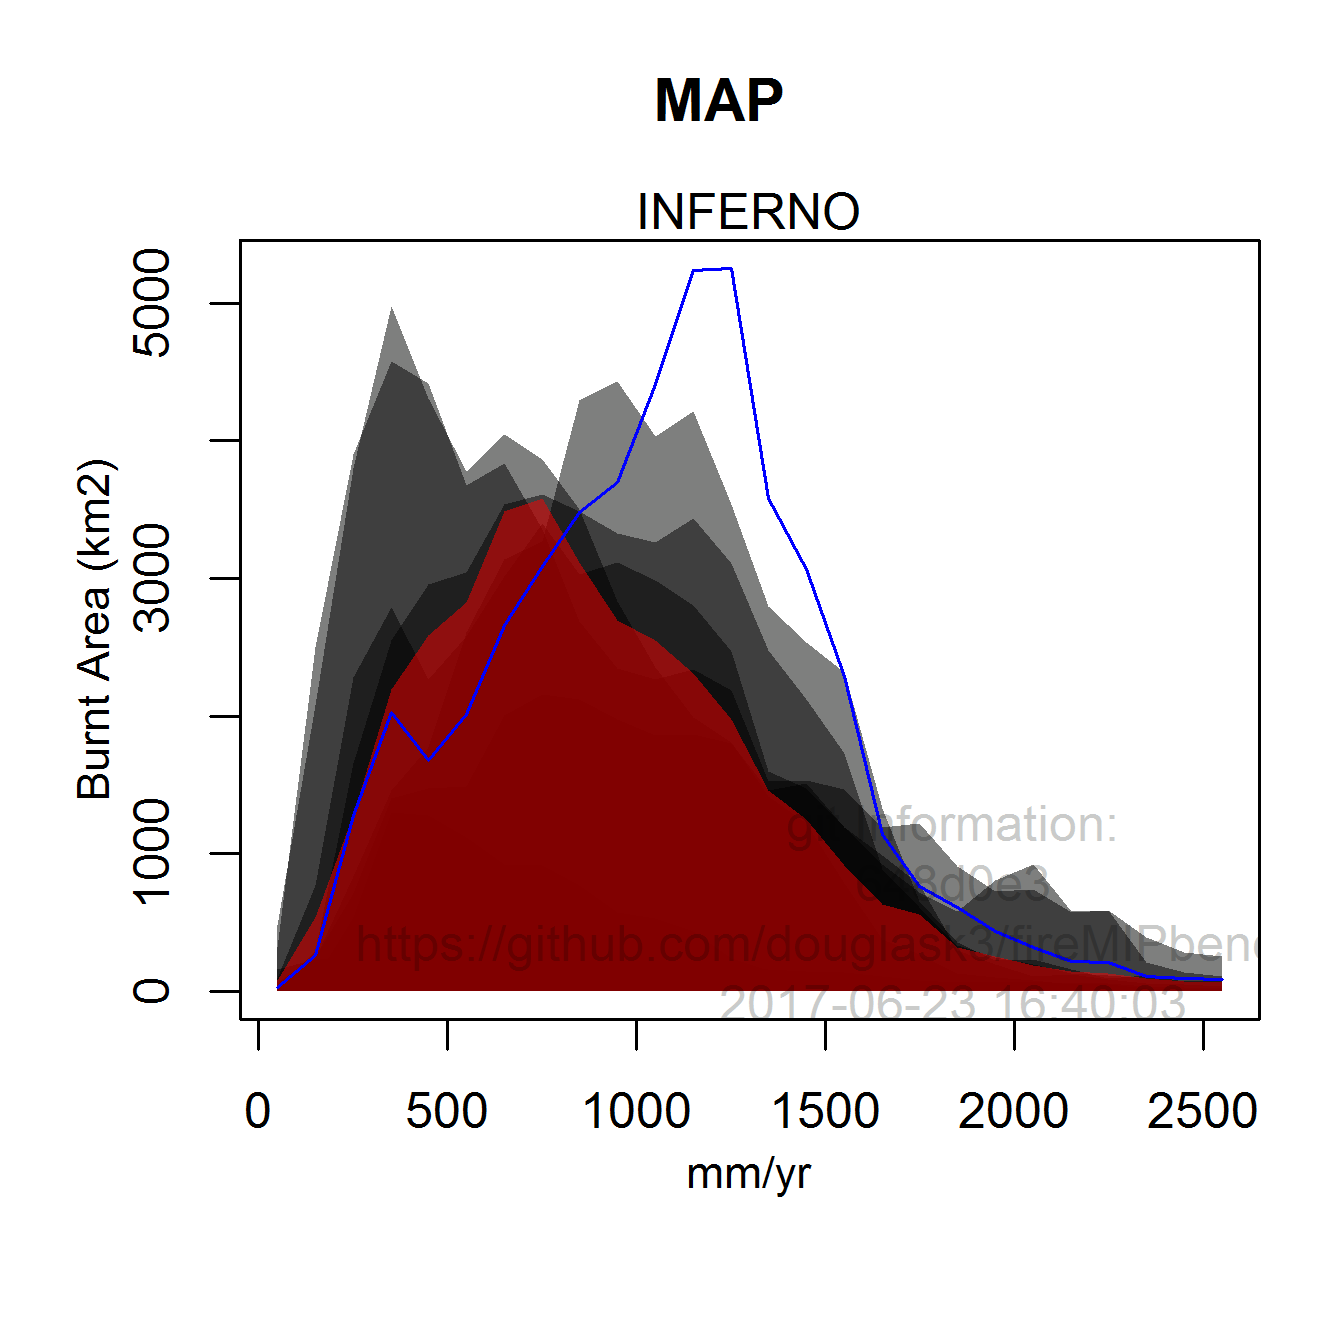
\includegraphics[width=4.8cm]{../../figs/burntArea_INFERNO_vs_MAP.png}	
	\end{textblock*}
	}
	\only<2->{
	\begin{textblock*}{14cm}(6.5cm,1.2cm)
		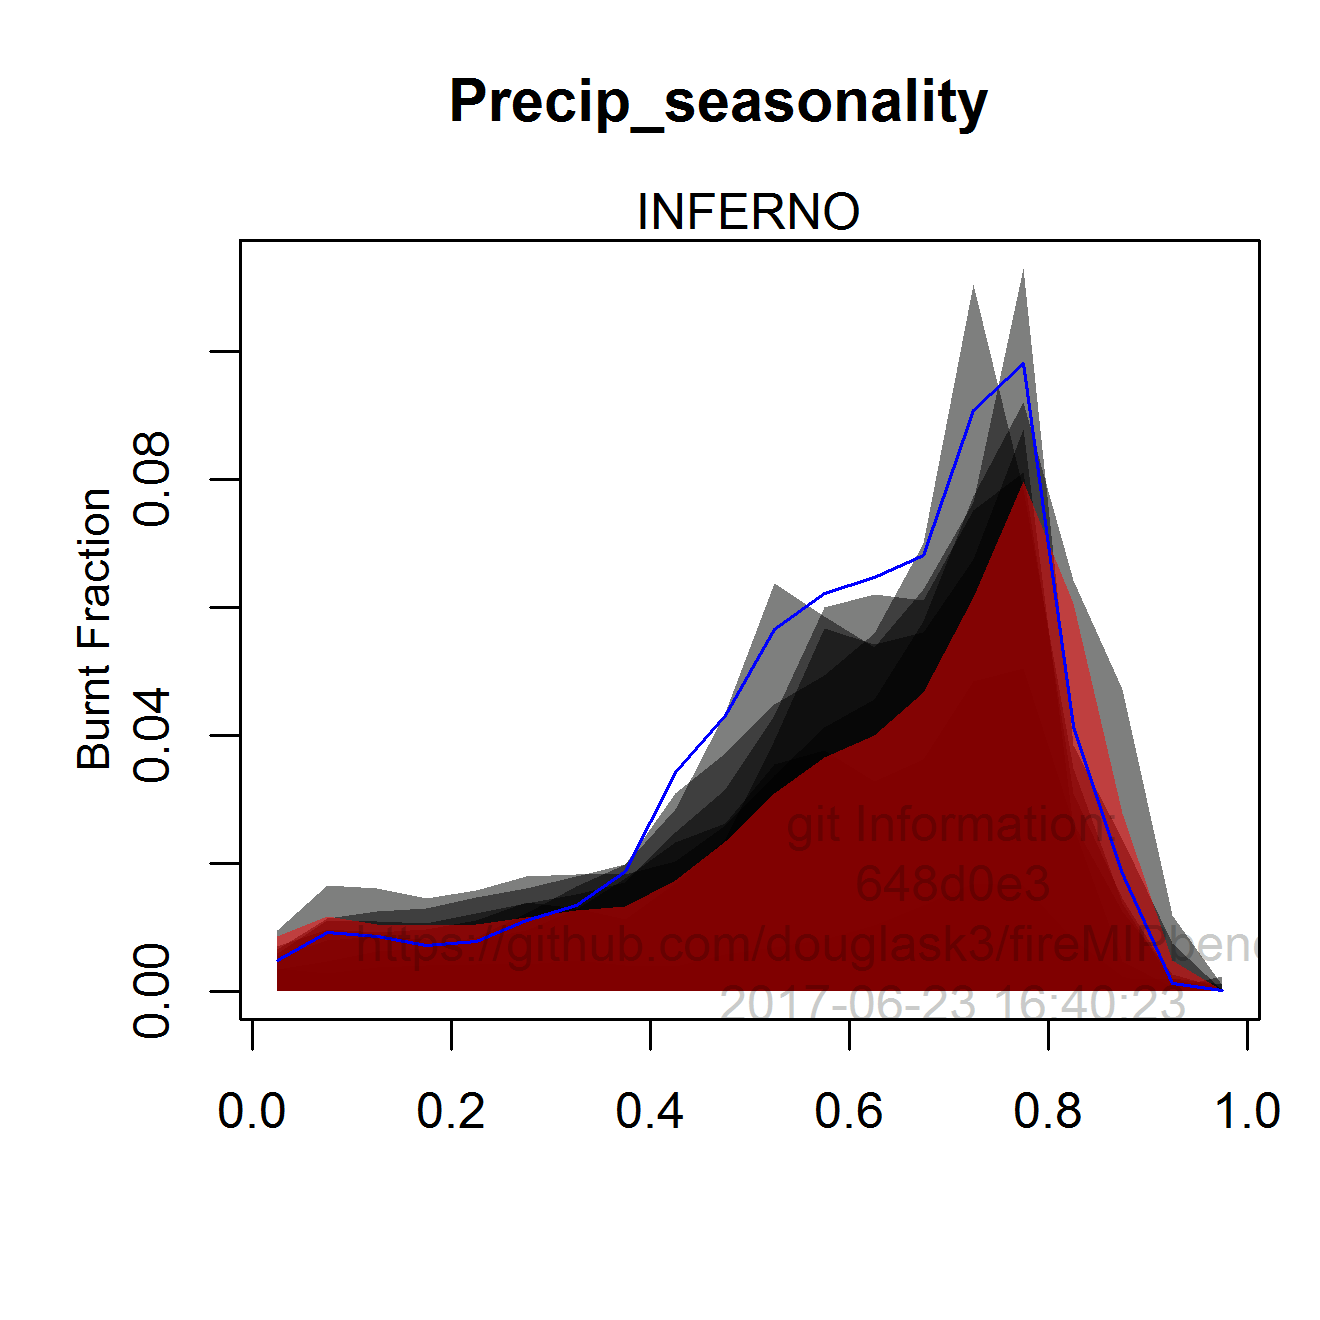
\includegraphics[width=4.8cm]{../../figs/burntArea_INFERNO_vs_Precip_seasonality.png}	
	\end{textblock*}
	}
	\only<3->{
	\begin{textblock*}{14cm}(3.4cm,4.5cm)
		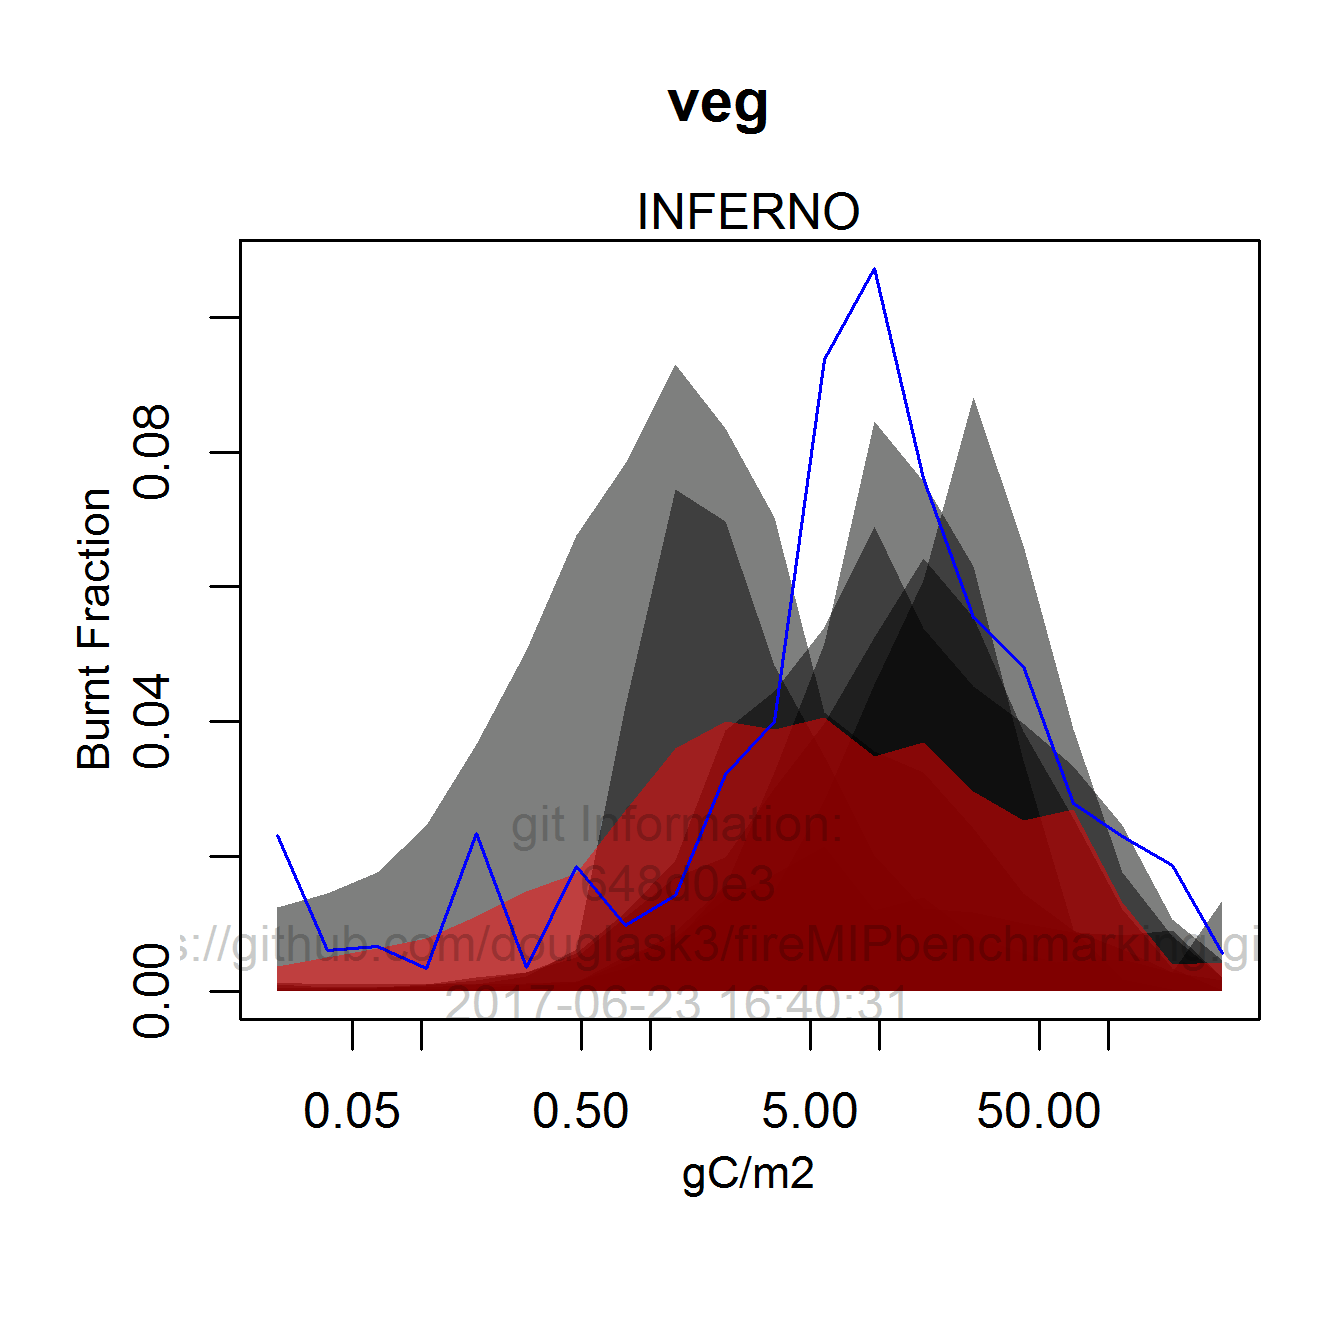
\includegraphics[width=4.8cm]{../../figs/burntArea_INFERNO_vs_veg.png}		
	\end{textblock*}
	}
	%\begin{textblock*}{14cm}(6.5cm,5.3cm)
	%	\includegraphics[width=5.78cm]{../diagrams/Logistic_fun.png}		
	%\end{textblock*}
\end{frame}


\begin{frame}
	\frametitle{INFERNO Seasonality}
	
\end{frame}

%Veg

